% -------------------------------------------------------------------------------------------------
%      MDSG Latex Framework
%      ============================================================================================
%      File:                  introduction-[UTF8,ISO8859-1].tex
%      Author(s):             Michael Duerr
%      Version:               1
%      Creation Date:         30. Mai 2010
%      Creation Date:         30. Mai 2010
%
%      Notes:                 - Example chapter
% -------------------------------------------------------------------------------------------------
%
\chapter{Einleitung}\label{sec:Introduction}
Dies ist der \LaTeX\ Rahmen zur Bearbeitung von Bachelor-, Master-, Projekt- und Diplomarbeiten.
Alle relevanten Dateien befinden sich im Verzeichnis \verb|text|.
\section{Unterverzeichnisse und Dateien}
Das Verzeichnis \verb|text| beinhaltet weitere Unterverzeichnisse und Dateien, die den Rahmen charakterisieren.
\subsection{\textbf{main.tex}}\label{subsec:main}
Diese Datei stellt die zentrale Konfigurationsdatei f�r den Rahmen dar. Unter anderem m�ssen hier Informationen
�ber die Aufgabensteller, Betreuer, die Art der Arbeit sowie deren Title eingestellt werden.
Hier k�nnen auch weitere Pakete eingebunden werden. Die Datei ist dokumentiert und sollte selbsterkl�rend
sein.
\subsection{\textbf{hyphenation.tex}}
Manche W�rter werden von \LaTeX\ nicht (ordentlich) getrennt. Diese k�nnen in dieser Datei mit deren
Trennungsstellen hinzugef�gt werden.
\subsection{\textbf{Makefile}}
Um das Dokument zu erstellen muss man den Aufruf \verb|make all| t�tigen. Dabei werden einige tempor�re
Dateien erstellt sowie die Datei \verb|main.pdf| die das entsprechende Dokument enth�lt. Mir dem
Aufruf \verb|make clean| werden alle tempor�ren Dateien sowie die Datei \verb|main.pdf| gel�scht.
sie k�nnen die Datei \verb|Makefile| ihren Anforderungen entsprechend erweitern.
\subsection{\textbf{text}}
Es bietet sich an f�r verschiedene Kapitel eigene Quelldateien zu pflegen. Diese sollten sie alle im
Ordner \verb|text| ablegen. Wie ein Kapitel eingebunden wird, kann man aus dem Beispiel in der
Datei \verb|main.tex| ablesen. Das Verzeichnis \textbf{text} beinhaltet zudem die Datei
\verb|abstract.tex|. In diese Datei soll eine kurze Zusammenfassung (ca. eine halbe Seite)
der Arbeit eingetragen werden. Die Datei \verb|appendix.tex| kann verwendet werden um einen
Anhang zu generieren.
\subsection{\textbf{pictures}}
Hier m�ssen sie alle Grafiken ablegen, die sie in ihrem Dokument einbinden wollen. Es sind nur die
Formate PDF, PNG und JPEG erlaubt (GIF ist m�glich, wird aber nicht empfohlen).
\subsection{\textbf{bibliography.bib}}
In diese Datei m�ssen alle Referenzen eingetragen werden,
die innerhalb ihrer Arbeit zitiert werden. Verwenden sie zur Verwaltung ihrer Referenzen einen
geeigneten Editor z.B. \textit{JabRef} (\url{http://jabref.sourceforge.net/}).
\subsection{\textbf{mdsg.sty}}
Hierbei handelt es sich um das Stylefile, das das Erscheinungsbild des Dokuments
lenkt. In dieser Datei sollten in der Regel keine Ver�nderungen notwendig sein.
\section{Beispiele}
Es gibt eine Unmenge an \LaTeX\ Tutorials und Dokumentationen, die guten Einstieg in das Arbeiten mit
\LaTeX\ erm�glichen. Im Folgenden werden aber ein paar undokumentierte Minimalbeispiele gegeben, die
den direkten Einstieg erm�glichen. Betrachten sie den Quelltext, um die Beispiele nachzuvollziehen.
\subsection{Zitate}
Wir zitieren hier eine Quelle von James Aspnes et al \cite{aspn07}, die in der  Datei\\
\verb|bibliography.bib|
steht.
\subsection{Listen}
Es gibt verschiedene M�glichkeiten Listen zu erstellen, z.B. ohne Nummerierung\dots
\begin{itemize}
   \item
      Das ist der erste Punkt,
      \begin{itemize}
         \item
            das der erste Unterpunkt,
         \item
            das der zweite Unterpunkt,
   \end{itemize}
   \item
      das der zweite, und
   \item
      das der dritte Punkt.
\end{itemize}
\dots oder mit Nummerierung\dots
\begin{enumerate}
   \item
      Das ist der erste Punkt,
      \begin{enumerate}
         \item
            das der erste Unterpunkt,
         \item
            das der zweite Unterpunkt,
      \end{enumerate}
   \item
      das der zweite, und
   \item
      das der dritte Punkt.
\end{enumerate}
\subsection{Referenz auf anderen Text}
Es ist auch m�glich auf andere Stellen im Text z.B. Kapitel \ref{subsec:main} zu verweisen.
\subsection{Hoch- und tiefgestellter Text}
Man kann Text tiefstellen indem man \verb|\textsubscript| verwendet, z.B. ergibt
\begin{verbatim}
text\textsubscript{tiefgestellt}
\end{verbatim}
den Text text\textsubscript{tiefgestellt}.
Das selbe funktioniert mit \verb|\textsuperscript| verwendet, z.B. ergibt
\begin{verbatim}
text\textsuperscript{hochgestellt}
\end{verbatim}
text\textsuperscript{hochgestellt}
\subsection{Tabellen}
Es gibt sch�ne M�glichkeiten Tabellen einzubinden wie z.B. Tabelle \ref{tab:CommonParameterSettings}.
\begin{center}
\begin{table}[htbp]
{\small
\begin{center}
\begin{tabular}[center]{lrlc}
\toprule
Parameter & Value & (Unit) & Available for Chord \\
\midrule
Query timeout & 10 & seconds & $\surd$ \\
Republish timeout & 300 & seconds & $\surd$ \\ % explain this value...
Stabilize timeout & 5 & seconds & $\surd$ \\
Fix fingers timeout & 30 & seconds & $\surd$ \\
Message timeout & 1 & second & $\surd$ \\
Connect timeout & 10 & seconds & $\surd$ \\
Ping superpeer timeout & 5 & seconds & $\times$ \\
Cost-Optimality estimation timeout & 20 & seconds & $\times$ \\
Significance for change in number of superpeers & 10 & percent & $\times$ \\
Significance for change in estimations  & 10 & percent & $\times$ \\
Number of permanent superpeers & 32 & nodes & $\times$ \\
Mean number of peers & 1000 & nodes & $\surd$ \\
Mean number of lookups per hour & 60 & queries & $\surd$ \\
Mean number of shared InfoProfiles per node & 20 & & $\surd$ \\
Identifier space & 16 & bits & $\surd$ \\
Direct insertion acknowledgment & true & bool & $\times$ \\
Direct query responses & true & bool & $\times$ \\
Force query resolution & true & bool & $\surd$  \\
\bottomrule
\end{tabular}
\end{center}
} % end of tiny
\caption[Simulation parameter settings]{Common simulation parameter settings.\label{tab:CommonParameterSettings}}
\end{table}
\end{center}

\subsection{Bilder}
Man kann sehr einfach Bilder einbinden so wie z.B. in Abbildung \ref{fig:pic0}.
\begin{figure}[hpbt]
  \centering
  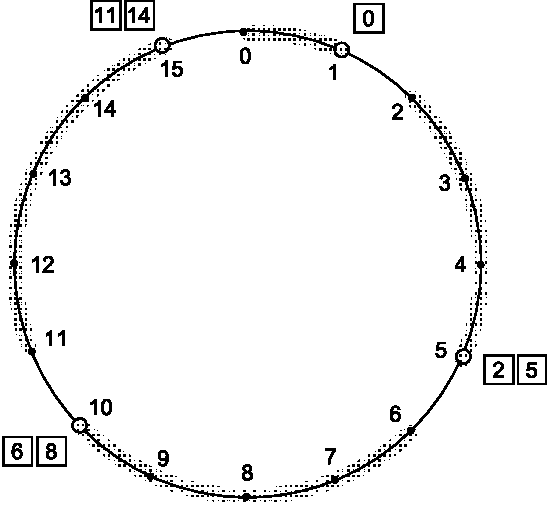
\includegraphics[width=0.4\textwidth]{pictures/pic0}\\
  \caption[Example of a $4$-bit Chord identifier circle]{Example of a $4$-bit Chord identifier circle.
  The responsibility ranges for each peer are accentuated in light gray}\label{fig:pic0}
\end{figure}
Es lassen sich auch mehrere Bilder nebeneinander platzieren wie z.B. in Abbildung
\ref{fig:multipic} zu sehen ist.
\begin{figure}[hpbt]
 \centering
  %%----start of first subfigure----
  \subfloat[FIFO size limited to 20 entries]{
   \label{fig:multipic:a} %% label for first subfigure
   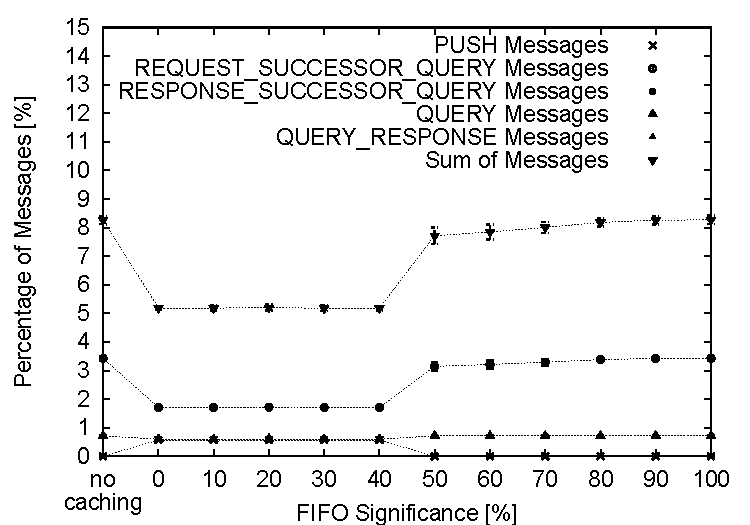
\includegraphics[width=0.48\linewidth]{pic1}}
  \hspace{0.01\textwidth}
  %%----start of second subfigure----
  \subfloat[FIFO size limited to 30 entries]{
   \label{fig:multipic:b} %% label for second subfigure
   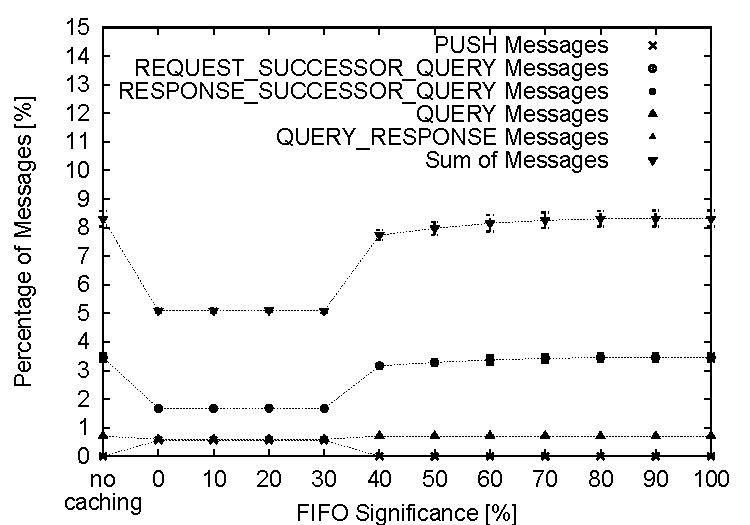
\includegraphics[width=0.48\linewidth]{pic2}}\\[0pt] % horizontal break
  %%----start of third subfigure----
  \subfloat[FIFO size limited to 40 entries]{
   \label{fig:multipic:c} %% label for third subfigure
   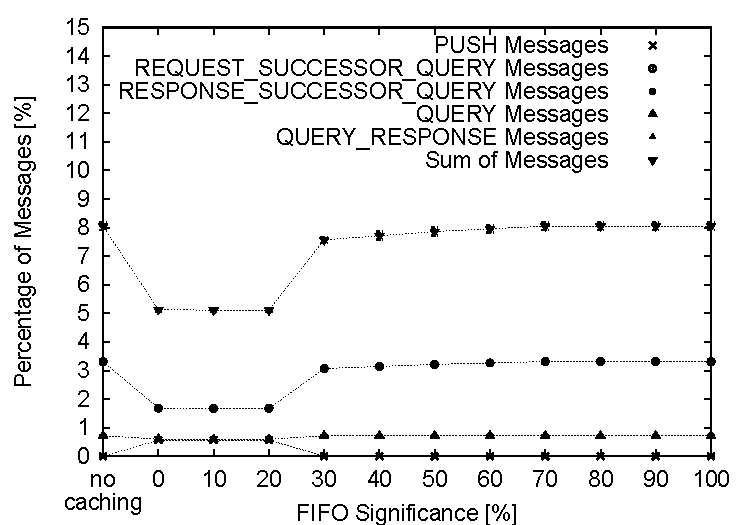
\includegraphics[width=0.48\linewidth]{pic3}}
  \hspace{0.01\textwidth}
  %%----start of fourth subfigure----
  \subfloat[FIFO size limited to 50 entries]{
   \label{fig:multipic:d} %% label for fourth subfigure
   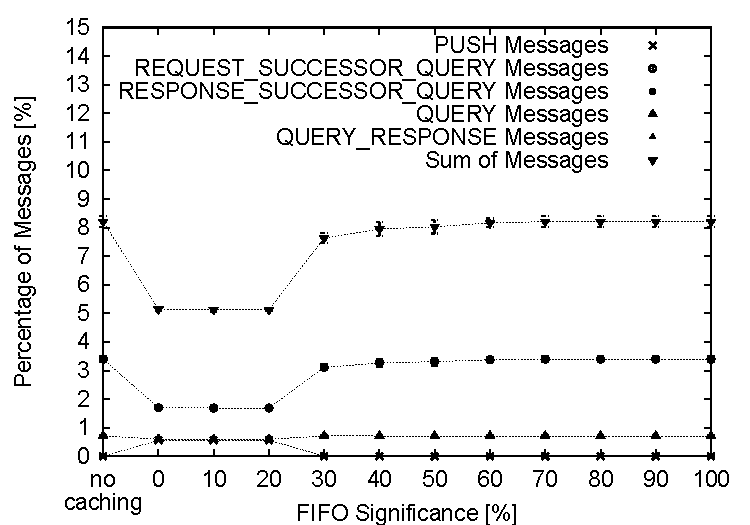
\includegraphics[width=0.48\linewidth]{pic4}}
 \caption[Observed message fractions and 95\% confidence intervals for Chord]{Observed message fractions and 95\% confidence intervals for Chord without the influence of churn. The FIFO capacity varies from 20 (\ref{fig:multipic:a}) -- 50 (\ref{fig:multipic:d}) entries (decadic steps).}
 \label{fig:multipic} %% label for entire figure
\end{figure}

\subsection{Programm Code}
Eine elegante M�glichkeit, Programmtext einzubinden, l�sst sich mit dem listings-Paket erreichen.
Das \verb|HelloWorld| Programm aus Listing \ref{lst:hw} hat in Zeile \ref{line:hw3} �brigens einen Programmierfehler.
\begin{lstlisting}[float=htp,caption=Hello World,label=lst:hw,language=Java, numbers=left, numberstyle=\tiny, stepnumber=2, numbersep=8pt, escapeinside={//@}{@//},backgroundcolor=\color{yellow},xleftmargin=3ex,xrightmargin=1ex]
public class HelloWorld {
    public static void main(String[] args) {
        Syste.out.println("Hello, World"); //@\label{line:hw3}@//
    }
}
\end{lstlisting}

\subsection{Fu�noten}
Wenn man auf Google \footnote{\url{http://www.google.com}} verweisen will, bietet sich statt einer gesonderten
Referenz auch einfach eine Fu�note an.
\subsection{Formeln}
Man kann mit \LaTeX\ sehr sch�n Formeln erzeugen:
$$L_{P}(k) = R^{orig}_{P}(k) + \sum_{i=0}^n 2*R^{i}_{P}(k)$$
